\section{Проектирование}
\subsection{Общая часть}
Задачей общей части проекта является: выявление и анализ структуры системы, разделение на индивидуальные части, определение взаимосвязей между ними. В языке UML для описания начальных стадий проекта чаще всего используются диаграммы вариантов использования, концептуальные диаграммы классов и сценарии. 

Диаграмма прецедентов (Use case diagram, диаграмма вариантов использования)~-- диаграмма, на которой отражены отношения, 
существующие между актерами и прецедентами.
Основная задача~-- представлять собой единое средство, дающее возможность заказчику, конечному пользователю и разработчику совместно
обсуждать функциональность и поведение системы.

Сущности, с которыми взаимодействует система в процессе своей работы, называются актерами или ролями, причем каждый актер ожидает, 
что система будет вести себя строго определенным, предсказуемым образом. В качестве ролей могут выступать человек или 
другая система, подсистема или класс, которые представляют нечто вне сущности.
Прецедент (use-case)~-- описание отдельного аспекта поведения системы с точки зрения пользователя.
В данном проекте диаграмма прецедентов выглядит так:

\begin{figure}[ht]
\centering
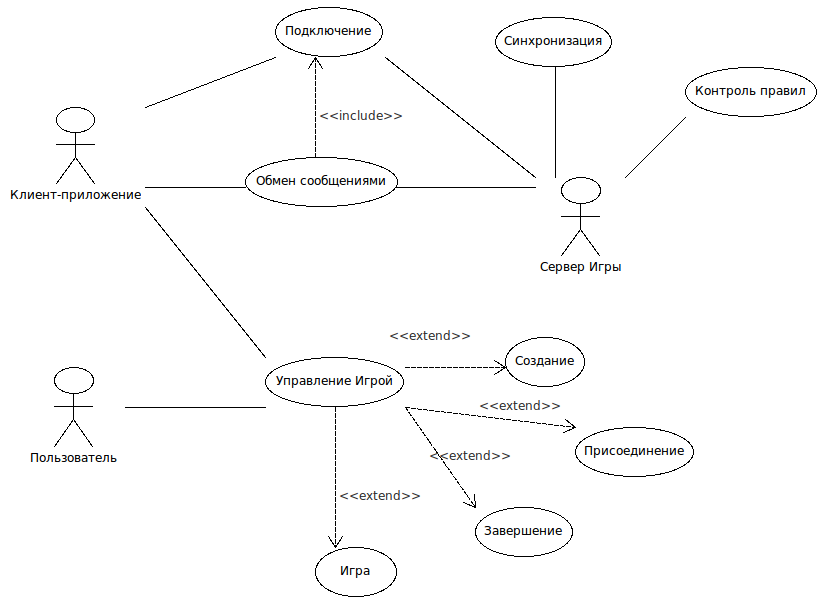
\includegraphics[width=18cm]{images/use.png}
\caption{Диаграмма прецедентов}
\label{fig0}
\end{figure}

На данной диаграмме [\ref{fig0}] видно, что взаимодействие игроков осуществляется через сервер игры, который
занимается синхронизацией(т.~е. чтобы игроки видели перемещения кораблей друг друга)
и проверкой соответствия их действий правилам игры. Под ролью пользователя на ней понимается 
человек, который использует данное приложение(графический интерфейс программы).

Клиенту должны быть доступны возможности создания и завершения игры, а так же управление самим процессом. Всё это вместе объединено под единым вариантом использования, названным <<Управление Игрой>>. Контроль произведенных операций осуществляется отдельной сущностью(сервером). Третий актер несет вспомогательную роль и является посредником между пользователем и сервером. У него должны иметься интерфейсы как графический, так и для общения с серверной частью. 

Прецеденты, являются действием или набором действий, выполняемых той или иной ролью. Прецедент может быть описан разными способами: диаграммой последовательности, диаграммой кооперации или сценарием.
Анализ требований и структуры системы показал, что целесообразно разделить проект на три составляющие, которые образуют основу концептуальной диаграммы классов. 
\begin{itemize}
	\item Взаимодействие клиента и сервера; 
	\item Клиент;
	\item Сервер;
\end{itemize} 

Концептуальной диаграммой классов называют диаграмму классов, в которой не раскрыты детальные отношения, связи, атрибуты и операции. Таким образом в этом типе диаграмм классов отражаются только основные связи между обобщёнными частями проекта. На рисунке [\ref{fig1}] представлена не развернутая диаграмма классов с концептуальной точки зрения.
\begin{figure}[ht]
\centering
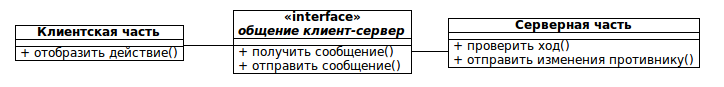
\includegraphics[width=17cm]{images/class.png}
\caption{Концептуальная диаграмма классов (а)}
\label{fig1}
\end{figure}

Проанализировав данную диаграмму [\ref{fig1}], было принято решение её детализировать, выделив на ней группы классов и те части проекта, которые непосредственно должны реализовывать описанный интерфейс. Стоит обратить внимание, что такие классы должны быть как в клиентской, так в серверной частях [\ref{fig2}].

\begin{figure}[ht]
\centering
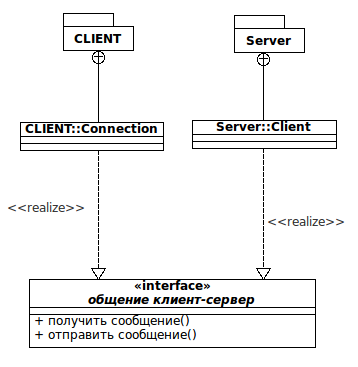
\includegraphics[width=9cm]{images/class1.png}
\caption{Концептуальная диаграмма классов (б)}
\label{fig2}
\end{figure}

Помимо диаграммы классов представлена диаграмма активностей [\ref{fig}], на которой отражена схема совершения хода системой в целом. Главная задача этой диаграммы показать, что действия игрока не отображаются в графическом интерфейсе напрямую и не ожидают подтверждения сервера, а вносятся тогда и только тогда, когда приходит команда от сервера. В случае неправильной команды будет отослано сообщение об ошибке. 

\begin{figure}[ht]
\centering
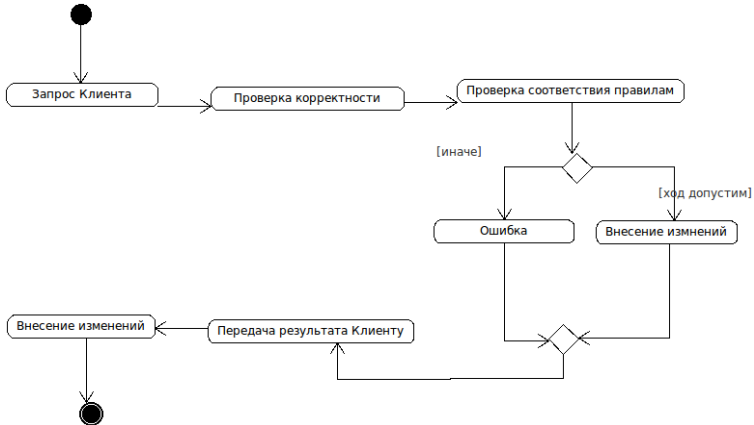
\includegraphics[width=15cm]{images/activitygen.png}
\caption{Схема хода игрока}
\label{fig}
\end{figure}


\endinput
